\chapter{\texorpdfstring{Search for extended Higgs sector signatures in $\PGt^+\PGt^-\PGt^+\PGt^-$ final states}{Search for extended Higgs sector signatures in tautautautau final states}}
\chaptermark{Extended Higgs sector search}  
\thispagestyle{plain}  % First page has default style
\pagestyle{chapterpages}
\label{Section:Chapter_4tau}
\minitoc

\section{Introduction}

Motivated by the theoretical considerations and the particularly intriguing measurement of the muon anomalous magnetic moment discussed in Section~\ref{Section:Chapter2_gminus2}, this chapter presents a detailed analysis targeting final states with four tau leptons $\PGt$ through the process $Z^*\rightarrow\phi A\rightarrow4\PGt$.

The analysis explores a region of parameter space that remains largely unconstrained by existing collider searches. This is primarily because the production mode proceeds via an off-shell $Z^*$ boson. This circumvents the dominant SM Higgs production mechanisms, which are already tightly constrained by current LHC measurements. As such, this search offers unique sensitivity to scenarios in extended Higgs sectors that could otherwise evade detection.

This chapter provides a comprehensive description of the analysis strategy employed in the CMS experiment to probe this signature. 
\section{Data and Simulation}
\subsection{Collision data}

This search is based on pp collision data collected by the CMS detector during the 2016-2018 Run 2 data-taking period. The collisions were recorded at a centre-of-mass energy $\sqrt{s} = 13\TeV$ and the full dataset corresponds to an integrated luminosity of approximately $138\unit{fb}^{-1}$.

\subsection{Backgrounds}

This section provides a brief overview of the SM processes that can contribute to the four-$\PGt$ signal region. The aim is to provide an understanding of how different backgrounds can enter the selection through the presence of genuine or misidentified $\PGt$ leptons. The specific treatment of each background category is described in detail in Section~\ref{Section:Chapter6_Background_Modelling}.

\textit{Diboson} production, specifically $\PZ\PZ \to 4\PGt$, constitutes the primary irreducible background in this analysis. These events contain four genuine $\PGt$ leptons in the final state, matching the signal topology by construction. Although the cross section is small compared to other SM processes, the kinematic features of $\PZ\PZ$ events make them difficult to distinguish from potential signal. In addition, $\PZ\PZ$ events with mixed-flavour decays can contribute irreducibly when the final state includes leptonic tau decays, such as $\PGt_e\PGt_e\PGt_h\PGt_h$ or $\PGt_\mu\PGt_\mu\PGt_h\PGt_h$. In such cases, the prompt electrons or muons from the $\PZ$ decay could mimic the kinematic signature of non-prompt leptons originating from $\PGt$ decays.

The \textit{\ac{DY}} process, $\PZ/\gamma^* \to \ell^+\ell^-$, is one of the dominant backgrounds in di-$\PGt$ final states, producing genuine $\PGt^+ \PGt^-$ pairs in approximately one-third of events. Although its impact is reduced in four-$\PGt$ final states, it remains relevant in cases where two genuine $\PGt$ leptons are produced and are accompanied by jets from ISR or FSR. These jets can be misidentified as $\PGt_h$ candidates, resulting in final states that pass the selection for four reconstructed $\PGt$ leptons. In addition, prompt electrons or muons from $\PZ/\gamma^* \to \Pe^+\Pe^-$ or $\mu^+\mu^-$ decays may be misidentified as $\PGt_h$ candidates. When combined with one or more jets that are also misidentified as $\PGt_h$, such events can satisfy the four-$\PGt$ selection criteria. Feynman diagrams illustrating DY production with and without ISR/FSR are shown in Figure~\ref{Figure:Chapter6_DY}.

\begin{figure}[h]
    \centering
    % First row
    \begin{subfigure}{0.45\textwidth}
        \centering
        \begin{tikzpicture}
    \begin{feynman}
        \vertex at (0, 1.5) (i1) {\(q\)};
        \vertex at (0,-1.5) (i2) {\(\overline{q}\)};

        \vertex at (2,0) (a);
        \vertex at (4, 0) (b);

        \vertex at (6.15, 1.5) (c) {\(\ell^-\)};
        \vertex at (6,-1.5) (d) {\(\ell^+\)};

        \vertex at (3,0.25) () {\(Z/\gamma^*\)};

        \diagram*{
            (i1) -- [fermion] (a) -- [fermion] (i2),
            (a) -- [photon] (b),
            (d) -- [fermion] (b) -- [fermion] (c),
        };
    \end{feynman}
\end{tikzpicture}
        \caption{}
    \end{subfigure}
    \hfill
    \begin{subfigure}{0.45\textwidth}
        \centering
        \begin{tikzpicture}
    \begin{feynman}
        \vertex at (0, 1.5) (i1) {\(q\)};
        \vertex at (0,-1.5) (i2) {\(\overline{q}\)};

        \vertex at (1.35, 0.5) (g1);
        \vertex at (2.5, 1.5) (g2);

        \vertex at (2,0) (a);
        \vertex at (4, 0) (b);

        \vertex at (6.15, 1.5) (c) {\(\ell^-\)};
        \vertex at (6,-1.5) (d) {\(\ell^+\)};

        \vertex at (3,0.25) () {\(Z/\gamma^*\)};

        \diagram*{
            (i1) -- [fermion] (a) -- [fermion] (i2),
            (g1) -- [gluon] (g2),
            (a) -- [photon] (b),
            (d) -- [fermion] (b) -- [fermion] (c),
        };
    \end{feynman}
\end{tikzpicture}
        \caption{}
    \end{subfigure}

    \caption[Examples of Feynman diagrams for Drell-Yan without partons and one parton originating from initial state radiation.]{Examples of Feynman diagrams for Drell-Yan \textbf{(a)} without partons and \textbf{(b)} one parton originating from ISR.}
    \label{Figure:Chapter6_DY}
\end{figure}

\textit{Top quark pair production} ($\ttbar \to b\overline{b}W^+W^-$) can also lead to four-$\PGt$ final states when both $\PW$ bosons decay leptonically via $\PW \to \PGt \nu_\PGt$. This results in two genuine $\PGt$ leptons, while additional jets from the top decays can be misidentified as $\PGt_h$ candidates, thereby mimicking the four-$\PGt$ topology. Misidentification can also occur between tau decay modes; for example, a $\PGt_h$ may be reconstructed as $\PGt_e$ or $\PGt_\mu$, or vice versa. Furthermore, similar to the DY background, prompt electrons or muons originating from $\PW \to e/\mu \nu$ decays may be misidentified as $\PGt_h$ candidates. In such cases, when combined with genuine $\PGt$ leptons or additional misidentified jets, multiple misidentifications may result in an event satisfying the four-$\PGt$ selection criteria.

\textit{W+jets} events can contribute to the four-$\PGt$ signal region when the $\PW$ boson decays via $\PW \to \PGt \nu_\PGt$, producing a genuine $\PGt$ lepton, and the accompanying jets are misidentified as $\PGt_h$ candidates. Similar to $\ttbar$, additional contributions arise from misidentified prompt electrons or muons. Since these events typically contain only one genuine lepton, multiple jet misidentifications are again required to satisfy the four-$\PGt$ selection.

\textit{QCD-induced multijet} events can enter the signal region when multiple jets are simultaneously misidentified as $\PGt_h$ candidates. These events may also feature non-prompt electrons or muons from the decay of hadrons. Such leptons can be misidentified as genuine prompt leptons and reconstructed as $\PGt_e$ or $\PGt_\mu$ candidates, thereby mimicking tau decays.

\textit{Diboson} processes such as $\PW\PW$ and $\PW\PZ$ may contribute to the four-$\PGt$ signal region when one or more of the bosons decay leptonically via $\PW/\PZ \to \PGt$, yielding up to two or three genuine $\PGt$ leptons. To satisfy the selection, the remaining $\PGt$ candidates must arise from jets misidentified as $\PGt_h$, originating either from hadronic boson decays (e.g., $\PW \to q \bar{q}'$, $\PZ \to q \bar{q}$) or from ISR or FSR. Misidentification of prompt electrons or muons as $\PGt_h$ candidates, following the same mechanism described for DY, $\ttbar$, and W+jets backgrounds, can also contribute. \textit{Triboson} production (e.g., $\PW\PW\PZ$, $\PZ\PZ\PZ$) can similarly yield multiple genuine leptons, including $\PGt$ decays, and may enter the signal region through analogous misidentification pathways.

Other subdominant processes also contribute. \textit{Single-top} production may yield a genuine $\PGt$ from a $\PW \to \PGt \nu_\PGt$ decay. Still, due to the typically low jet multiplicity in these events, additional $\PGt_h$ candidates must arise from misidentified jets, often requiring ISR or FSR. Finally, \textit{electroweak production} of $\PZ$ or $\PW$ bosons in association with jets (\eg VBF-like $\PZ + jj$) can resemble the signal topology when real or misidentified $\PGt$ candidates are produced alongside forward jets. 

Although many of the backgrounds discussed above are partially reducible through the application of $\PGt$ identification algorithms, lepton isolation requirements, and $b$-jet vetoes, these techniques are not fully efficient, and some backgrounds remain irreducible. To summarise, a common feature across many of these background processes is the presence of prompt electrons or muons that can be reconstructed as leptonic or hadronic $\PGt$ candidates. This, in combination with jet misidentification, enables events with fewer than four genuine $\PGt$ leptons to satisfy the selection criteria. The specific treatment, estimation, and validation of each background category are described in detail in Section~\ref{Section:Chapter6_Background_Modelling}.

The simulated background processes used in this analysis are summarised in Table~\ref{Table:Chapter6_SimulatedBackgrounds}.

{
\centering
\setlength{\LTpost}{-2ex}  % tighten space after table
\small  % one size smaller than normal
\begin{longtable}{llc}
\caption[Summary of the simulated Standard Model backgrounds, including their generators and precision, used in the extended Higgs sector search.]
{Summary of the simulated SM backgrounds, including their generators and precision, used in the search. The following generators were used: 
\MADGRAPH~\cite{MadGraph} for leading-order matrix element calculations; 
\POWHEG~v1.0~\cite{Powheg_0} and v2.0~\cite{Powheg_1,Powheg_2,Powheg_3} for next-to-leading order processes including $\ttbar$ and single top; 
and \MGvATNLO~\cite{MadGraph} for diboson and triboson production. 
Parton showering and hadronisation were performed with \PYTHIA~\cite{PYTHIA}.}
\label{Table:Chapter6_SimulatedBackgrounds} \\
\hline
\textbf{Process} & \textbf{Generators} & \textbf{Cross section $\sigma$ [pb]} \\
\hline \hline
\endfirsthead

\hline
\textbf{Process} & \textbf{Generators} & \textbf{Cross section $\sigma$ [pb]} \\
\hline \hline
\endhead

\hline
\multicolumn{3}{r}{\textit{Continued on next page}} \\
\endfoot

\hline
\endlastfoot
\rowcolor{verylightblue}
\textbf{Drell-Yan, $\PZ/\gamma^* \to \ell^+ \ell^-$ (LO)\hyperlink{DY_W-MLM}{$^1$}} & & \\
+ jets, $10 < m_{\ell \ell} < 50\GeV$ & \MADGRAPH, \PYTHIA & 15810.0 (LO), 18610.0 (NLO) \\
+ jets, $m_{\ell \ell} > 50\GeV$ & \MADGRAPH, \PYTHIA & 5379.0 (LO), 6077.2 (NNLO) \\
+1 jets\hyperlink{DY_W-Stitch}{$^2$}, $m_{\ell \ell} > 50\GeV$ & \MADGRAPH, \PYTHIA & 997.3 (LO) \\
+2 jets\hyperlink{DY_W-Stitch}{$^2$}, $m_{\ell \ell} > 50\GeV$ & \MADGRAPH, \PYTHIA & 347.0 (LO)\\
+3 jets\hyperlink{DY_W-Stitch}{$^2$}, $m_{\ell \ell} > 50\GeV$ & \MADGRAPH, \PYTHIA & 126.4 (LO) \\
+4 jets\hyperlink{DY_W-Stitch}{$^2$}, $m_{\ell \ell} > 50\GeV$ & \MADGRAPH, \PYTHIA & 71.7 (LO) \\

\arrayrulecolor{lightgray}\hline
\rowcolor{verylightblue}
\textbf{W+jets (LO)\hyperlink{DY_W-MLM}{$^1$}} & & \\
+ jets & \MADGRAPH, \PYTHIA & 52940.0 (LO), 61526.7 (NLO) \\
+1 jets\hyperlink{DY_W-Stitch}{$^2$} & \MADGRAPH, \PYTHIA & 9364.4 (LO) \\
+2 jets\hyperlink{DY_W-Stitch}{$^2$} & \MADGRAPH, \PYTHIA & 3168.6 (LO) \\
+3 jets\hyperlink{DY_W-Stitch}{$^2$} & \MADGRAPH, \PYTHIA & 1132.1 (LO) \\
+4 jets\hyperlink{DY_W-Stitch}{$^2$} & \MADGRAPH, \PYTHIA & 633.7 (LO) \\

\arrayrulecolor{lightgray}\hline
\rowcolor{verylightblue}
\textbf{\ttbar} & & \\
Fully hadronic & \POWHEG, \PYTHIA & 377.96 (NNLO)\\
Semi-leptonic & \POWHEG, \PYTHIA & 365.34 (NNLO)\\
Fully leptonic & \POWHEG, \PYTHIA & 88.29 (NNLO) \\

\arrayrulecolor{lightgray}\hline
\rowcolor{verylightblue}
\textbf{Single top} & & \\
t-channel ($t$) & \POWHEG, \PYTHIA & 136.02 (NNLO) \\
t-channel ($\overline{t}$) & \POWHEG, \PYTHIA & 136.02 (NNLO) \\
$t + W^-$ & \POWHEG, \PYTHIA & 35.60 (NNLO) \\
$t + W^+$ & \POWHEG, \PYTHIA & 35.60 (NNLO) \\

\arrayrulecolor{lightgray}\hline
\rowcolor{verylightblue}
\textbf{Diboson} & & \\
$\PW \PZ \rightarrow \ell \, \nu \, \nu \, \nu$  & \MCATNLO, \PYTHIA & 3.416 (NLO) \\
$\PW \PZ \rightarrow \ell \, \nu \, q \, q$        & \MCATNLO, \PYTHIA & 10.71 (NLO) \\
$\PW \PZ \rightarrow q \, q \, \ell \, \ell$            & \MCATNLO, \PYTHIA & 6.419 (NLO) \\
$\PW \PZ \rightarrow \ell \, \ell \,  \ell \, \nu $          & \MCATNLO, \PYTHIA & 5.213 (NLO) \\
$\PW \PW \rightarrow \ell \, \nu \, q \,q$        & \MCATNLO, \PYTHIA & 49.99 (NLO) \\
$\PW \PW \rightarrow \ell \, \nu \, \ell \, \nu$        & \POWHEG, \PYTHIA & 11.09 (NLO) \\
$\PZ \PZ \rightarrow \ell \, \ell \, \nu \, \nu$         & \POWHEG, \PYTHIA & 0.9740 (NLO) \\
\arrayrulecolor{lightgray}\hline
$\text{H}_{\text{VBF}} \rightarrow ZZ \rightarrow \ell \, \ell \, \ell \, \ell $ & \POWHEG, \PYTHIA & $1.040e^{-3}$ (NLO) \\
$\text{ggH} \rightarrow ZZ \rightarrow \ell \, \ell \, \ell \, \ell $ & \POWHEG, \PYTHIA & $1.333e^{-2}$ (NLO)\\
$qq \rightarrow ZZ \rightarrow \ell \, \ell \, \ell \, \ell $ & \POWHEG, \PYTHIA & 1.325 (NLO)\\
$gg \rightarrow ZZ \rightarrow e \, e \, \PGt \, \PGt $ & \PYTHIA & $3.194e^{-3}$ (NLO)\\
$gg \rightarrow ZZ \rightarrow \mu \, \mu \, \PGt \, \PGt $ & \PYTHIA & $3.194e^{-3}$ (NLO)\\
$gg \rightarrow ZZ \rightarrow \mu \, \mu \, \mu \, \mu $ & \PYTHIA & $1.585e^{-3}$ (NLO)\\
$gg \rightarrow ZZ \rightarrow \PGt \, \PGt \, \PGt \, \PGt $ & \PYTHIA & $1.585e^{-3}$ (NLO)\\

\arrayrulecolor{lightgray}\hline
\rowcolor{verylightblue}
\textbf{Triboson} & & \\
$\PW \PW \PZ $ & \MCATNLO, \PYTHIA & 0.1707 (NLO)\\
$\PW \PZ \PZ $ & \MCATNLO, \PYTHIA & 0.0571 (NLO)\\
$\PW \PW \PW $ & \MCATNLO, \PYTHIA & 0.2158 (NLO)\\
$\PZ \PZ \PZ $ & \MCATNLO, \PYTHIA & 0.0148 (NLO)\\

\arrayrulecolor{lightgray}\hline
\rowcolor{verylightblue}
\textbf{Pure Electroweak} & & \\
$\PW^+ \to \ell^+ \nu$ + 2 jets & \MADGRAPH, \PYTHIA & 25.62 (LO)\\
$\PW^- \to \ell^- \nu$ + 2 jets & \MADGRAPH, \PYTHIA & 20.25 (LO)\\
$\PZ \to \ell \ell$ + 2 jets & \MADGRAPH, \PYTHIA & 3.987 (LO)\\

\arrayrulecolor{black}\hline
\end{longtable}
}
{
\footnotesize
\begin{flushleft}
\hypertarget{DY_W-MLM}{}$^{1}$ MLM jet matching scheme~\cite{MLM} is employed to avoid double counting between jets produced at the matrix element level and those generated during parton showering. \\

\hypertarget{DY_W-Stitch}{}$^{2}$ To improve statistical precision, exclusive samples with fixed jet multiplicities are generated using the MLM scheme. These are stitched with inclusive samples to reproduce the overall cross-section and kinematic distributions accurately.
\end{flushleft}
% For \ac{NLO} simulations, however, the MLM scheme is incompatible with the negative event weights that naturally arise. In such cases, the FxFx jet merging scheme~\cite{FxFx} is used instead. 
}

% Although the background samples are generated at LO or NLO, the comparison of simulated events to data is performed using higher-order theoretical cross-sections. Specifically, $\PW$+jets, Z+jets, $\ttbar$, and single top quark events in the tW channel are normalised using \ac{NNLO} cross-sections~\cite{HighOrder_XS_1,HighOrder_XS_2,HighOrder_XS_3}, while single top and diboson events are normalised to cross-sections calculated at NLO~\cite{HighOrder_XS_3,HighOrder_XS_4,HighOrder_XS_5}.

\subsection{Modelling of Signal Processes}
\label{Section:Chapter6_SignalModelling}

Signal templates targeting the process $Z^* \to \phi A \to \PGt^+\PGt^-\PGt^+\PGt^-$ are modelled in the \MCATNLO (version 2.6.5) framework~\cite{MadGraph,FxFx} at NLO accuracy in QCD. The event generation is performed in the five-flavour scheme using the NNPDF3.1 PDFs~\cite{NNPDF}. Parton showering, hadronisation, and $\PGt$ lepton decays are simulated using \PYTHIA (version 8.230)~\cite{PYTHIA}, with the underlying event modelled according to the CP5 tune~\cite{CP5_Tune}. To reflect realistic running conditions, additional pp interactions are overlaid on simulated events according to the distribution observed in the Run 2 data-taking period. The detector response is simulated using the \GEANTfour-based CMS framework~\cite{GEANT4}, and events are reconstructed with the same software configuration as applied to collision data.

A two-dimensional mass grid is defined to ensure sensitivity across the allowed phase space. All masses are expressed in units of~\GeV. The grid consists of combinations of $m_A$ and $m_\phi$ as follows:

\begin{itemize}
    \item $m_A$: 40, 50, 60, 70, 80, 90, 100, 125, 140, 160, 200, 250, 300, 400, 600
    \item For each $m_A$, the following $m_\phi$ values are considered:
    \begin{itemize}
        \item $m_A = 40$--$90$: 60, 70, 80, 90, 100, 110, 125, 140, 160, 180, 200, 250, 300
        \item $m_A = 100$, $125$, $140$, $160$, $200$, $250$:  60-300 (as above), 400
        \item $m_A = 300$: 60–400 (as above), 600
        \item $m_A = 400$: 100, 110, 125, 140, 160, 180, 200, 250, 300, 400, 600
        \item $m_A = 600$: 400, 600, 800
    \end{itemize}
\end{itemize}

The signal is simulated under the \textit{alignment limit} of the 2HDM, consistent with current experimental constraints on the couplings of the observed Higgs boson. The specific scenario is dynamically selected at each mass point depending on the value of $m_\phi$:
\begin{itemize}
    \item For $m_\phi > 125~\GeV$, the heavier CP-even scalar is identified as $\phi \equiv H$
    \item For $m_\phi \leq 125~\GeV$, the lighter CP-even scalar is identified as $\phi \equiv h$
\end{itemize}

Model parameters that do not significantly influence the kinematic properties of the final state, such as the charged Higgs mass and the soft $\mathbb{Z}_2$-breaking term, are fixed to values that preserve perturbative unitarity. This also ensures theoretical consistency~\cite{TypeX_2HDM}. Variations of these parameters within their allowed ranges have negligible impact on the resulting signal kinematics. They are therefore set according to the following prescription:
\begin{equation_pad}
m_{H^\pm} = m_\phi, \quad\quad m_{12}^2 = m_\phi^2 \sin\beta \cos\beta.
\end{equation_pad}

Figure~\ref{Figure:Chapter6_GenVisDistributions} illustrates the generator-level distributions of the visible di-$\PGt$ mass for selected combinations of $m_\phi$ and $m_A$. This observable is defined as the invariant mass computed using only the visible decay products of the two $\PGt$ leptons (\ie excluding neutrinos). These examples illustrate the primary kinematic characteristics of the signal across the mass grid.

\begin{figure}[h]
        \centering
        % First row
        \begin{subfigure}[b]{0.49\textwidth}
            \centering
            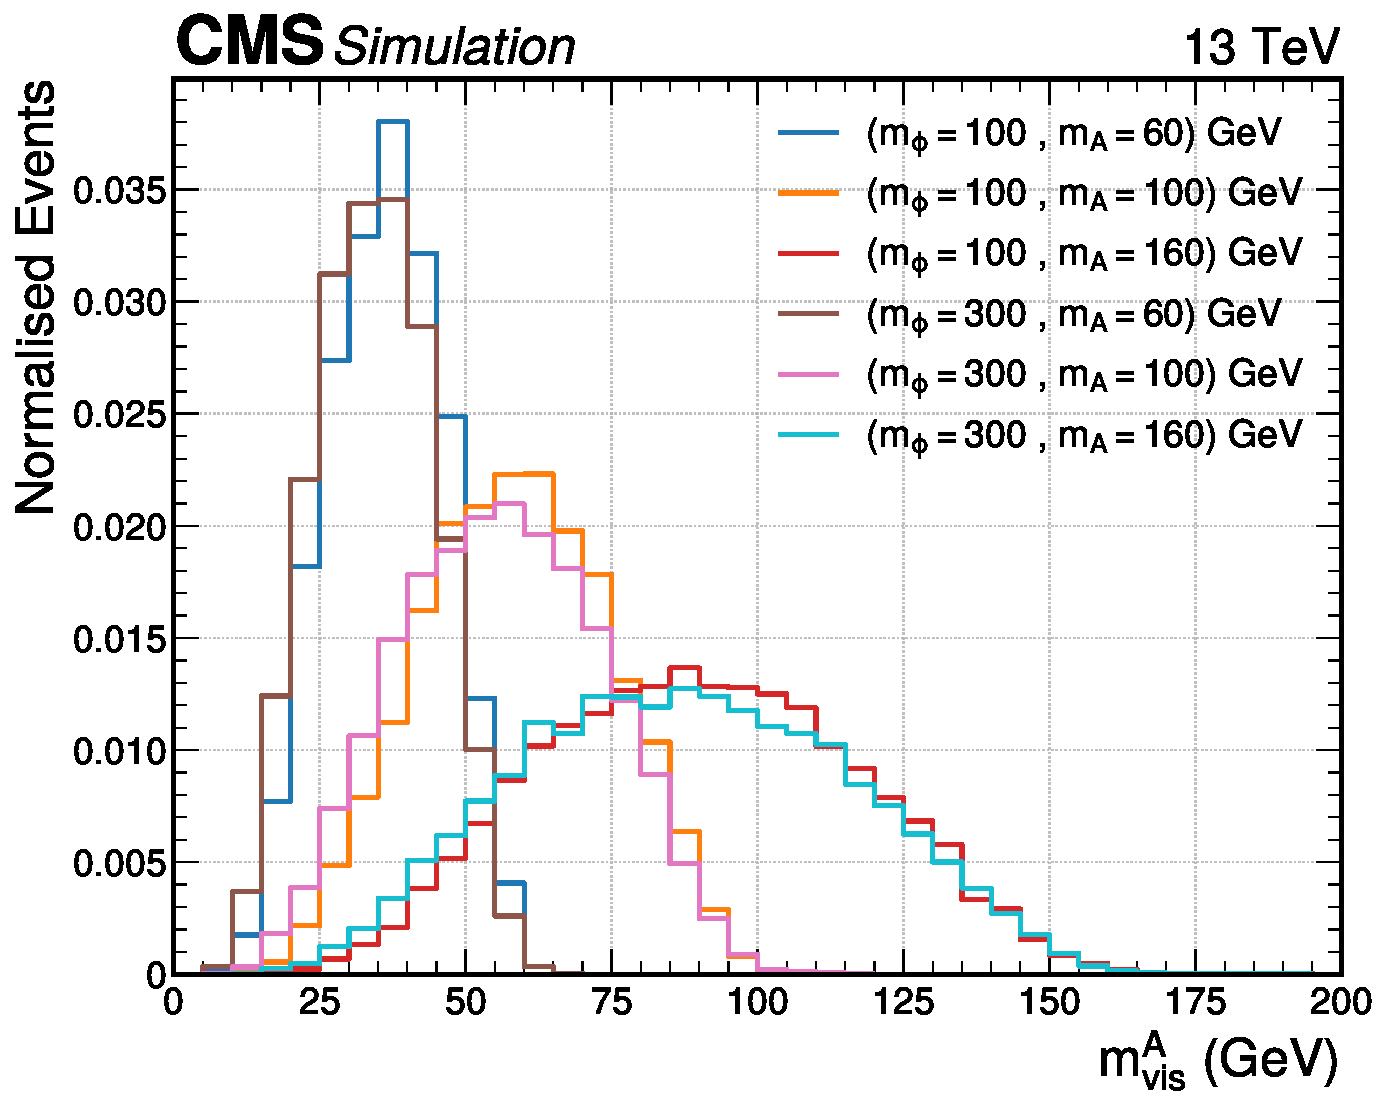
\includegraphics[width=\textwidth]{Figures/Chapter6/mvis_A.pdf}
            \caption{}
        \end{subfigure}
        \begin{subfigure}[b]{0.49\textwidth}
            \centering
            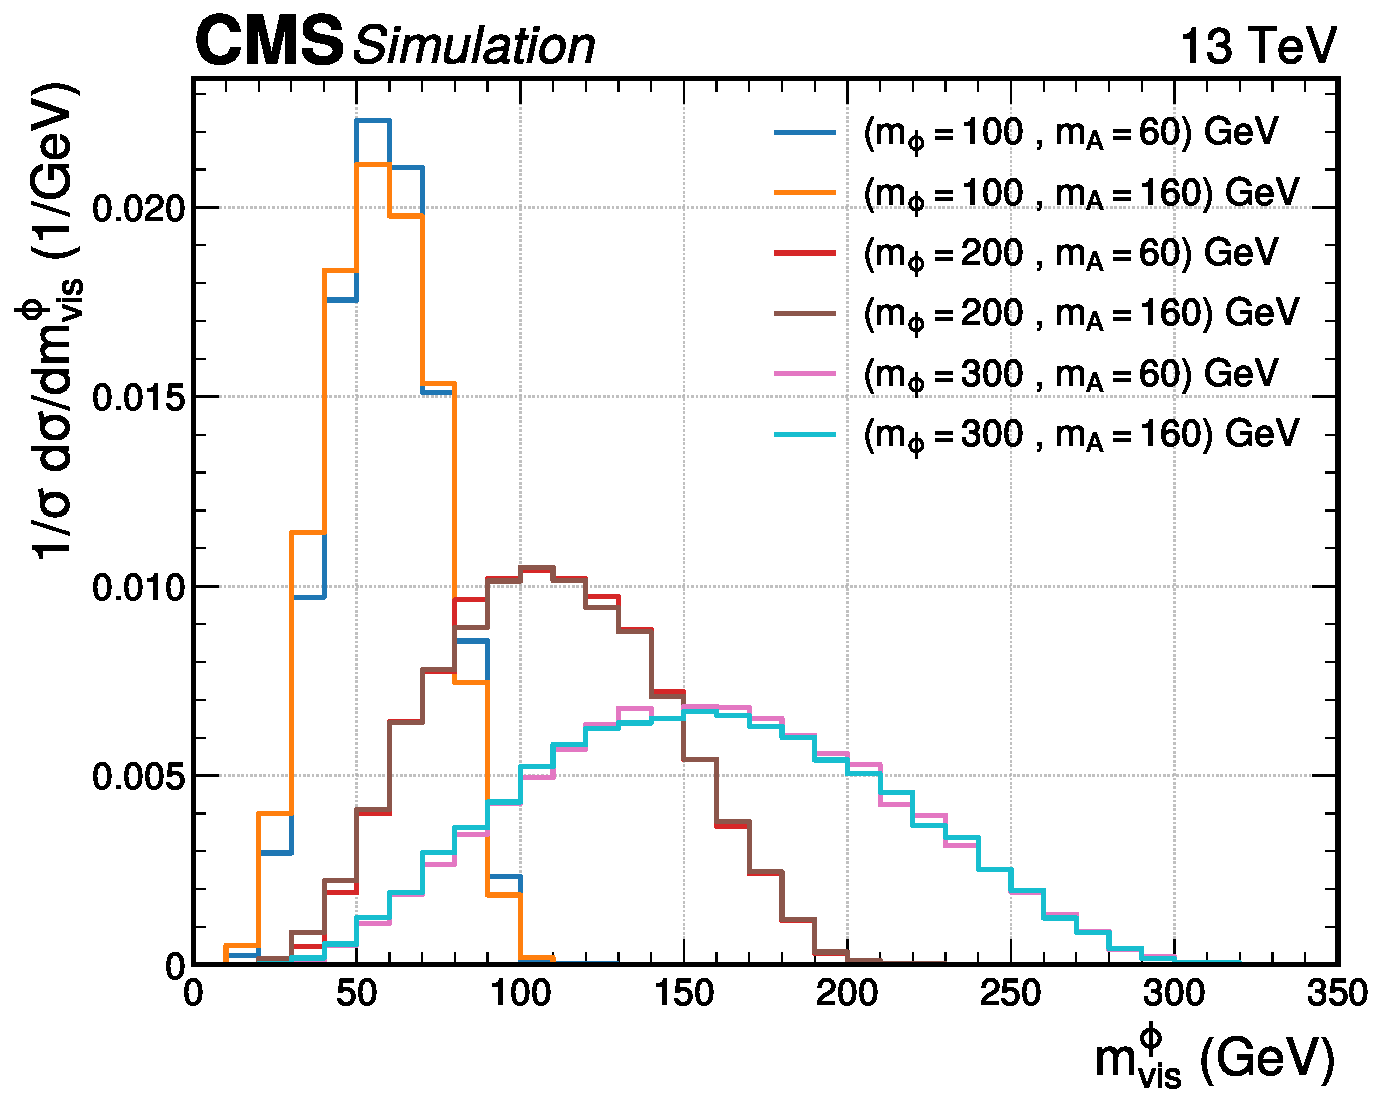
\includegraphics[width=\textwidth]{Figures/Chapter6/mvis_phi.pdf}
            \caption{}
        \end{subfigure}
    \caption[Generator-level visible mass distributions for selected mass points.]{Generator-level distributions of the visible di-$\PGt$ mass for selected combinations of $m_A$ and $m_\phi$. The visible mass is computed using only the decay products of the two $\PGt$ leptons, excluding neutrinos. Distributions are shown for scans over \textbf{(a)} $m_A$ and \textbf{(b)} $m_\phi$.}
    \label{Figure:Chapter6_GenVisDistributions}
\end{figure}

\subsubsection{Production Cross Sections and Branching Fractions}

The production cross section is computed at NLO and, within the alignment limit, is independent of $\tan\beta$. It varies across the mass plane, ranging from approximately $10~\unit{fb}$ at $(m_\phi, m_A) = (100, 60)~\GeV$ to $650~\unit{fb}$ at $(300, 160)~\GeV$. These values are summarised in Figure~\ref{Figure:Chapter6_ProductionXS}, which shows the cross section as a function of the two mass parameters in the alignment scenario.

\begin{figure}[htbp]
  \centering
  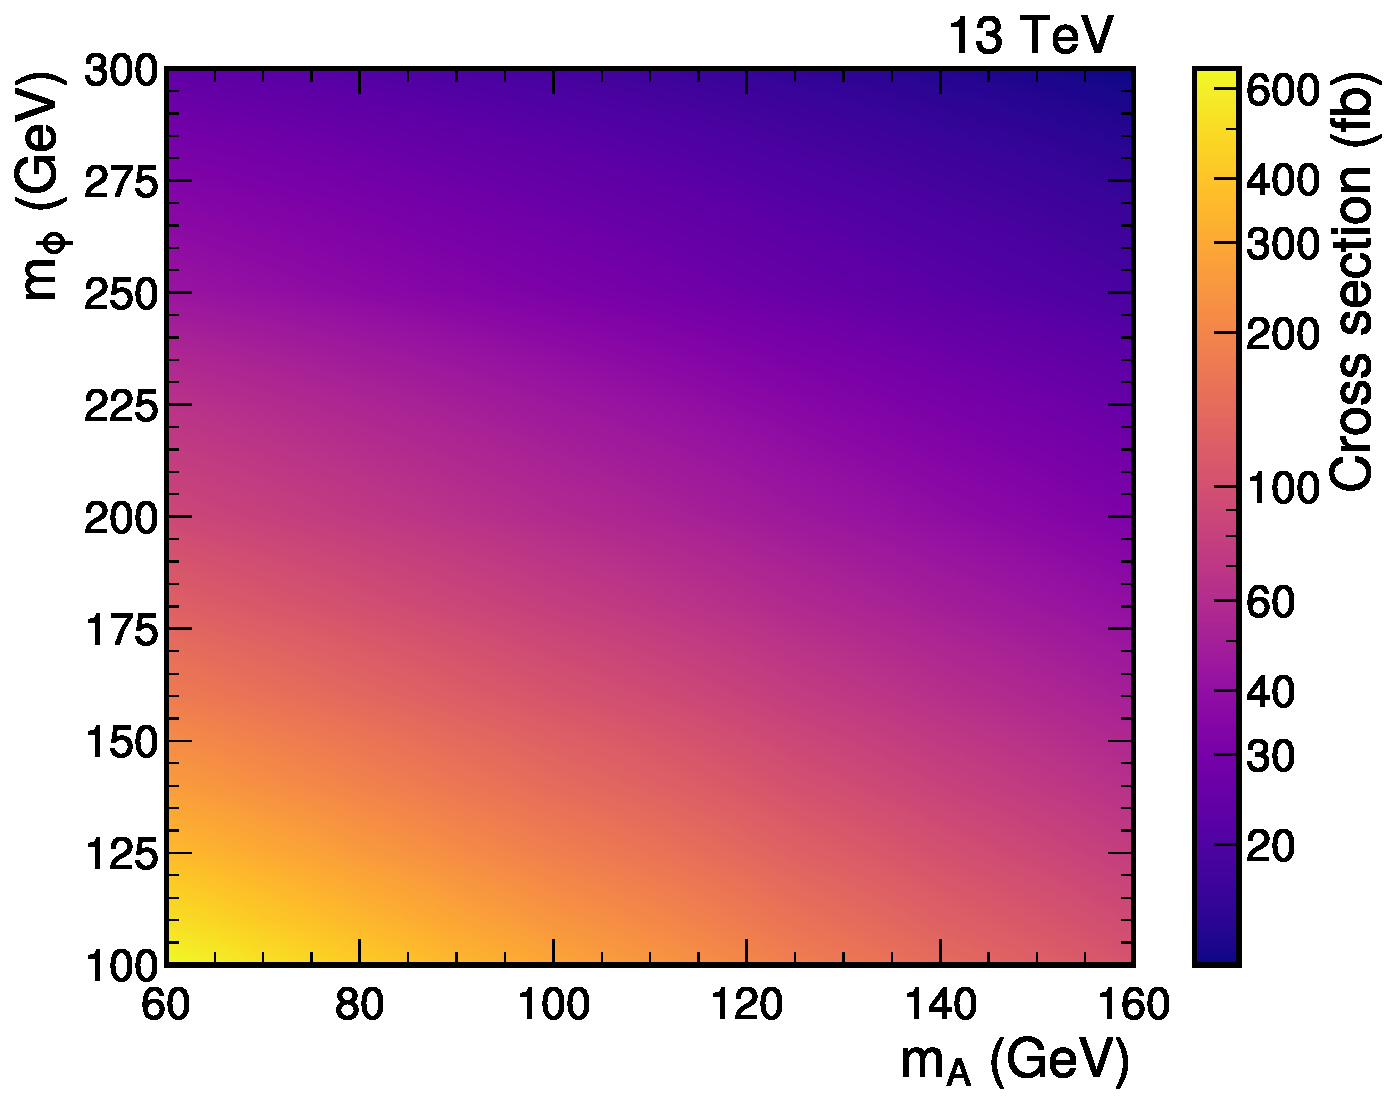
\includegraphics[width=0.75\textwidth]{Figures/Chapter6/Production_XS.pdf}
    \caption[Production cross sections for $Z^* \to \phi A$ in the alignment limit]{Production cross sections for $Z^ \to \phi A$ in the alignment limit at NLO, shown as a function of $m_\phi$ and $m_A$. The values are interpolated over a grid of simulated mass combinations.}
  \label{Figure:Chapter6_ProductionXS}
\end{figure}

Outside the alignment limit, the cross section acquires dependence on the scalar mixing angle. Specifically:
\begin{itemize}
    \item It scales with $\sin^2(\beta - \alpha)$ when $\phi \equiv H$ ($m_\phi > 125~\GeV$),
    \item It scales with $\cos^2(\beta - \alpha)$ when $\phi \equiv h$ ($m_\phi \leq 125~\GeV$).
\end{itemize}

The decay branching ratios of $\phi$ and $A$ into $\PGt^+\PGt^-$ are computed using \textsc{2HDECAY}~\cite{2HDECAY}. In the alignment limit, the $\PGt^+\PGt^-$ branching ratio of $A$ remains close to unity for $\tan\beta \gtrsim 2$, but decreases rapidly at lower $\tan\beta$, where hadronic decays such as $A \to b\bar{b}$ become dominant. A similar pattern holds for $\phi \to \PGt^+\PGt^-$, except when the mass difference $m_\phi - m_A$ exceeds $m_Z$. In such cases, the decay $\phi \to ZA$ becomes kinematically accessible and can significantly suppress the di-$\PGt$ branching fraction, even at large $\tan\beta$. These features are illustrated in Figure~\ref{Figure:Chapter6_BranchingFractions}, which shows representative branching fraction maps for selected mass configurations. 

\begin{figure}[h]
        \centering
        % First row
        \begin{subfigure}[b]{0.49\textwidth}
            \centering
            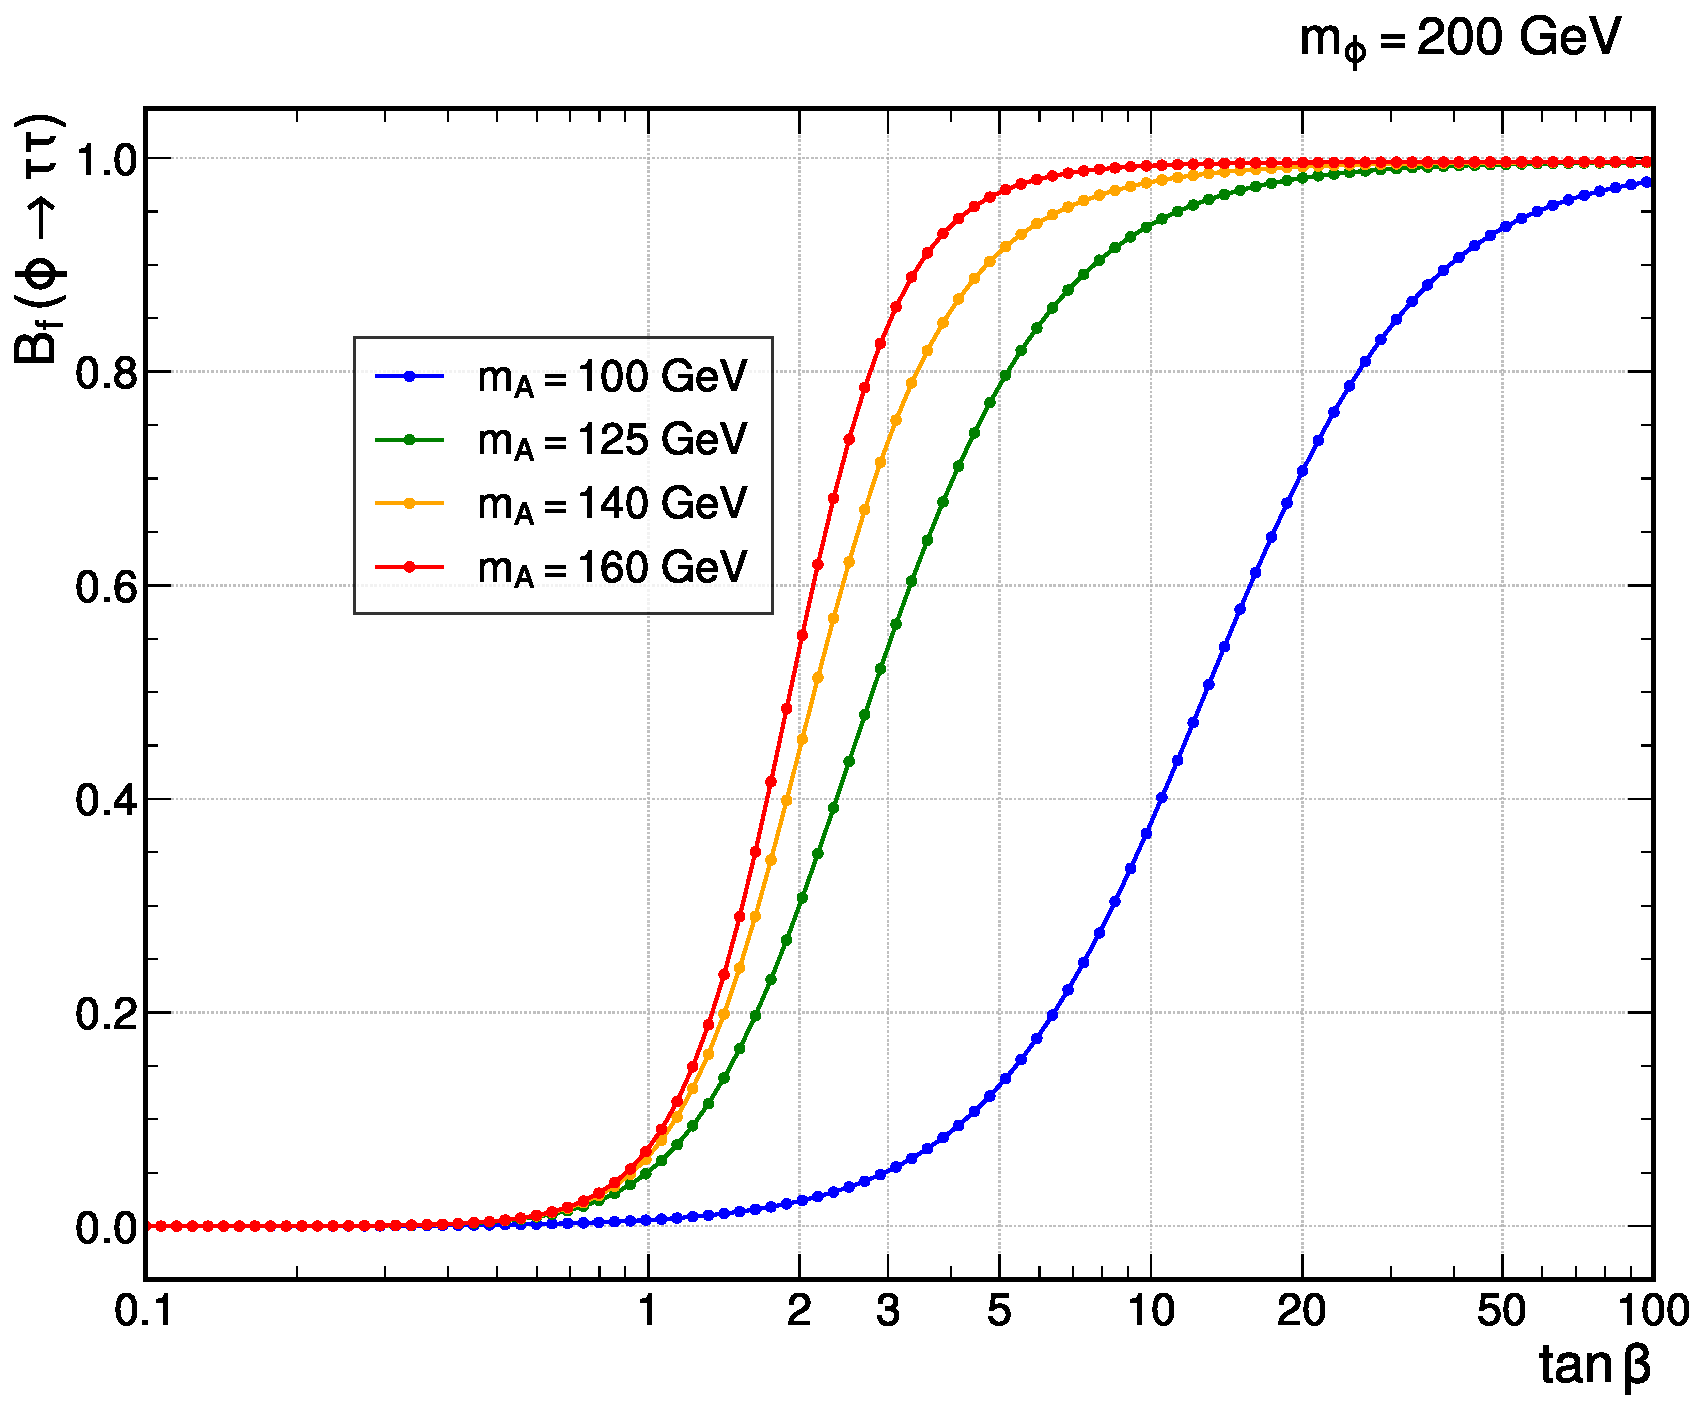
\includegraphics[width=\textwidth]{Figures/Chapter6/Phi_BR.pdf}
            \caption{}
        \end{subfigure}
        \begin{subfigure}[b]{0.49\textwidth}
            \centering
            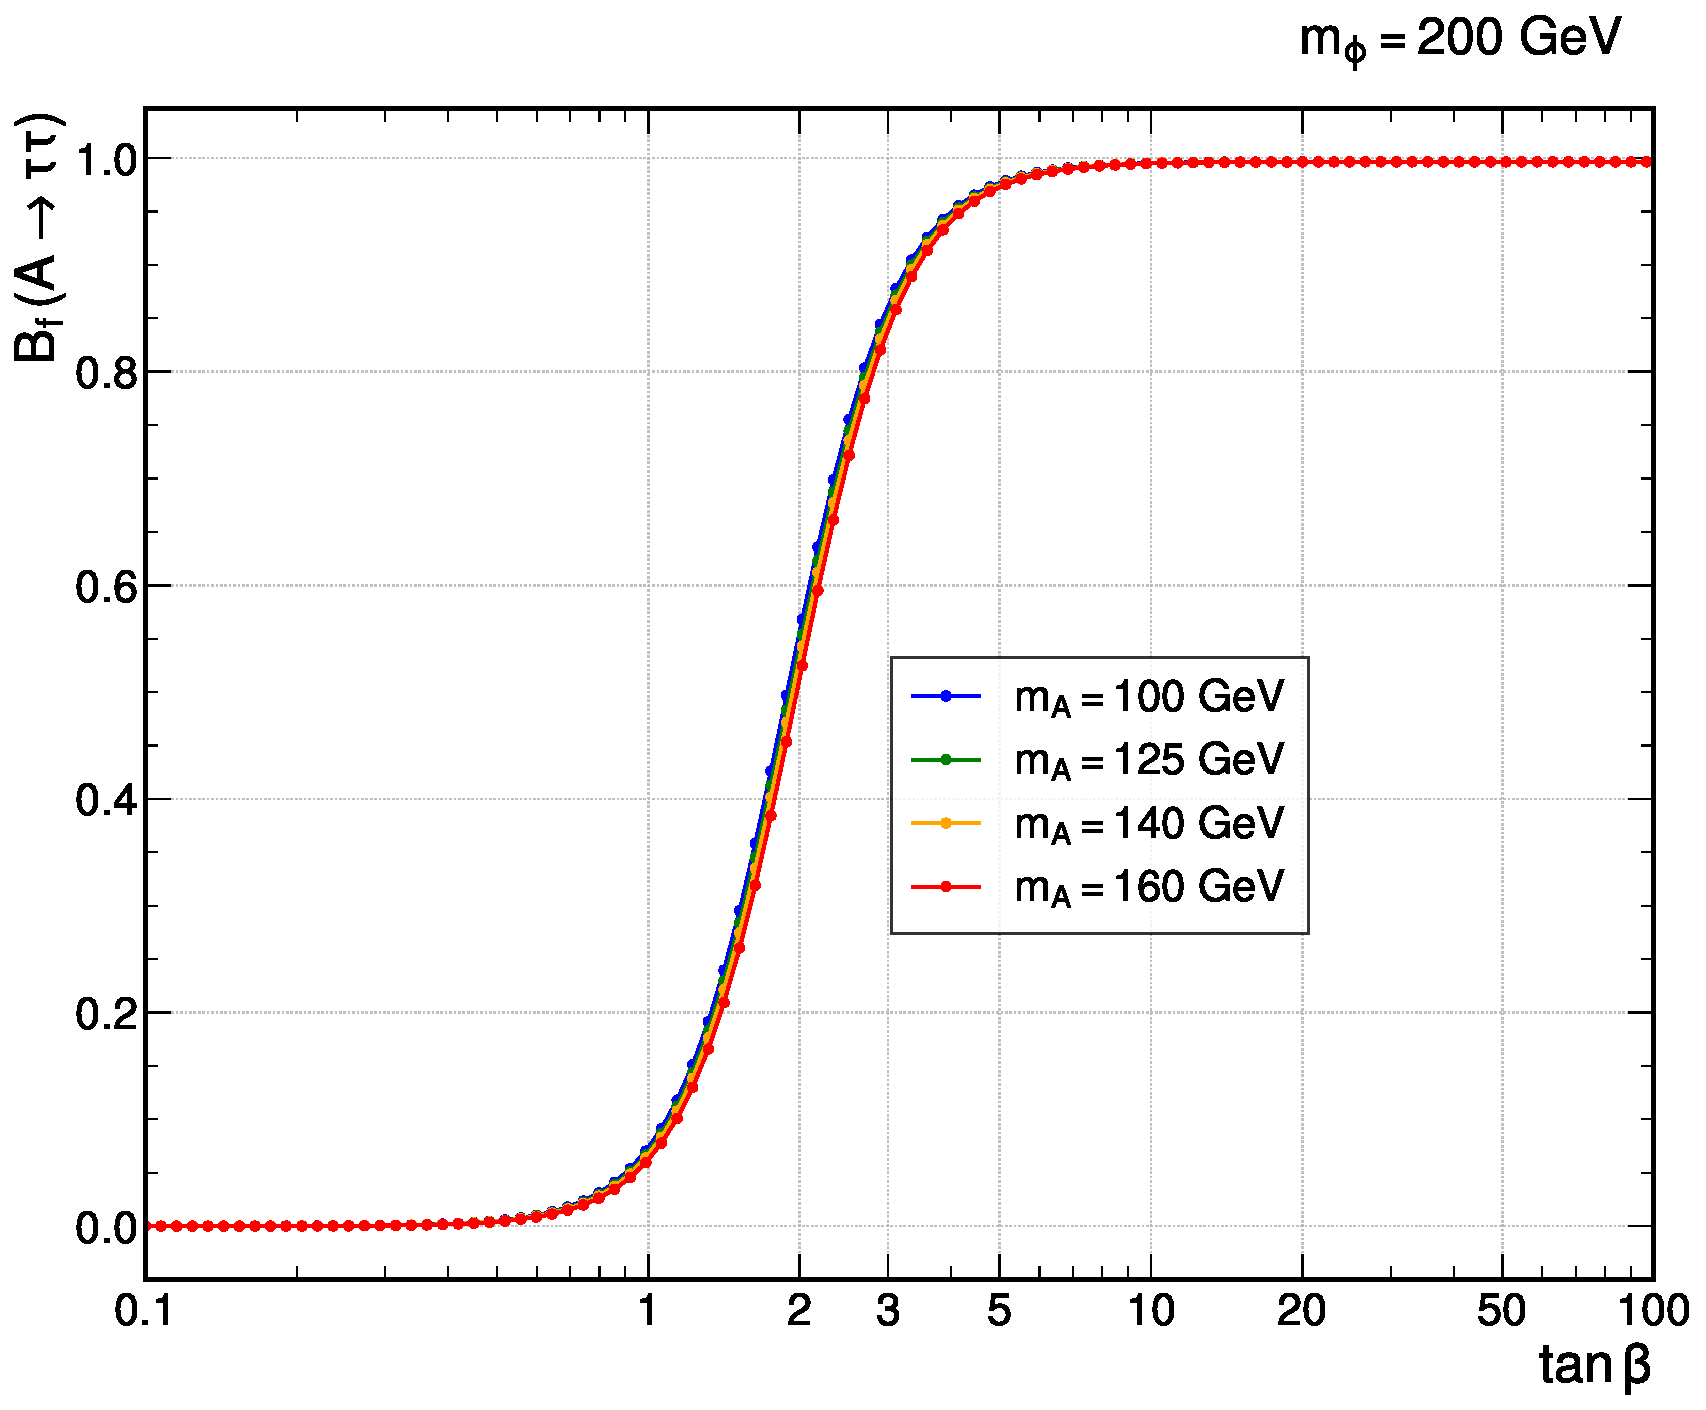
\includegraphics[width=\textwidth]{Figures/Chapter6/A_BR.pdf}
            \caption{}
        \end{subfigure}
    \caption[Branching fractions of $\phi$ and $A$ to $\PGt^+\PGt^-$ for selected mass combinations.]{Branching fractions of \textbf{(a)} $\phi \to \PGt^+\PGt^-$ and \textbf{(b)} $A \to \PGt^+\PGt^-$ as a function of $m_\phi$ and $m_A$, computed using \textsc{2HDECAY} in the alignment limit.}
    \label{Figure:Chapter6_BranchingFractions}
\end{figure}

\section{Object \& Event Selections}
\label{sec:ObjectAndEventSelections}

Having established the motivation, signal modelling, and background composition, this section describes the strategy used to identify candidate $Z^* \to \phi A \to 4\PGt$ events. The selection procedure aims to efficiently retain signal-like events while minimising contamination from dominant background processes and maximising the rejection of objects originating from PU interactions.

The final states considered consist of four tau leptons, each of which may decay either leptonically ($\PGt_e$ and $\PGt_{\mu}$) or hadronically ($\PGt_h$). Figure~\ref{Figure:Chapter6_4tau_decayModes_BF} displays a pie chart of the most frequent $4\PGt$ final states, constructed by enumerating all combinations of leptonic and hadronic tau decays and summing their relative contributions. The dominant modes are those containing two or more hadronic taus, which together comprise 87.1\% of all four-tau decays. These channels form the focus of the analysis. In contrast, Table~\ref{Table:Chapter6_4tau_decayModes_BF_Other} summarises rarer final states that are not considered in the analysis.

\begin{figure}[htbp]
  \centering
  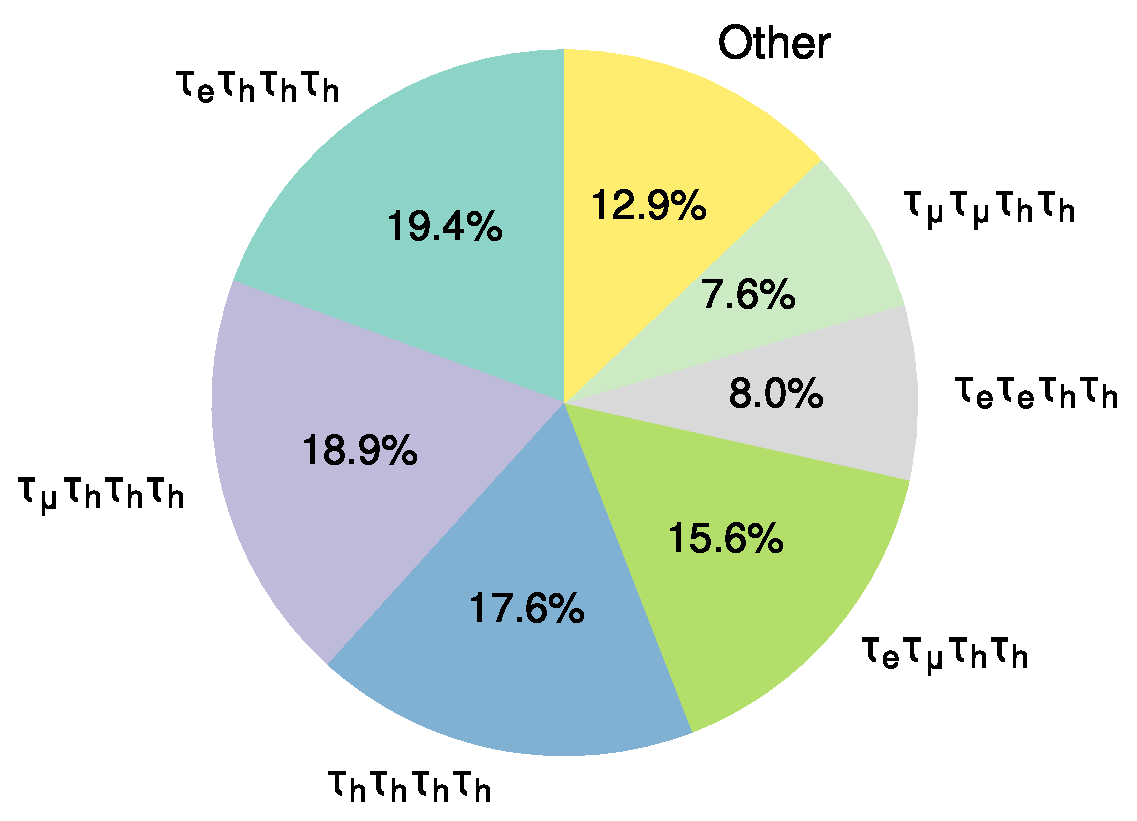
\includegraphics[width=\textwidth]{Figures/Chapter6/pie_BF.pdf}
    \caption[Production cross sections for $Z^* \to \phi A$ in the alignment limit]{Production cross sections for $Z^ \to \phi A$ in the alignment limit at NLO, shown as a function of $m_\phi$ and $m_A$. The values are interpolated over a grid of simulated mass combinations.}
  \label{Figure:Chapter6_4tau_decayModes_BF}
\end{figure}

\begin{table}[h]
\centering
\renewcommand{\arraystretch}{1.5} % Increase row height
\setlength{\tabcolsep}{12pt} % Increase column width
\arrayrulecolor{black} % Ensure outer border is black
\begin{tabular}{|c|c|}
\hline
Decay Mode                  & Branching Fraction {[}\%{]} \\ \hline \hline
$\PGt_e \PGt_e \PGt_{\mu} \PGt_h$             & 4.3 \\ 
\arrayrulecolor{lightgray} \hline
$\PGt_e \PGt_{\mu} \PGt_{\mu} \PGt_h$                    & 4.2 \\ 
\arrayrulecolor{lightgray} \hline
$\PGt_e \PGt_e \PGt_{e} \PGt_h$                        & 1.5  \\ 
\arrayrulecolor{lightgray} \hline
$\PGt_{\mu} \PGt_{\mu} \PGt_{\mu} \PGt_h$                  & 1.4  \\ 
\arrayrulecolor{lightgray} \hline
$\PGt_e \PGt_e \PGt_{\mu} \PGt_{\mu}$             & 0.6  \\ 
\arrayrulecolor{lightgray} \hline
$\PGt_e \PGt_e \PGt_{e} \PGt_{\mu}$                     & 0.4  \\ 
\arrayrulecolor{lightgray} \hline
$\PGt_e \PGt_{\mu} \PGt_{\mu} \PGt_{\mu}$             & 0.4  \\ 
\arrayrulecolor{lightgray} \hline
$\PGt_e \PGt_e \PGt_{e} \PGt_e$                  & 0.1  \\ 
\arrayrulecolor{lightgray} \hline
$\PGt_{\mu} \PGt_{\mu} \PGt_{\mu} \PGt_{\mu}$                  & 0.1  \\ 
\arrayrulecolor{black} \hline
\end{tabular}
\caption[Branching fractions of subdominant four-$\PGt$ decay modes]{Branching fractions of subdominant four-$\PGt$ final states, involving three or more leptonic $\PGt$ decays.}
\label{Table:Chapter6_4tau_decayModes_BF_Other}
\end{table}

\subsection{Physics Object Selection}
\label{sec:ObjectSelection}

All reconstructed objects are derived from the CMS particle-flow (PF) algorithm, which combines tracking and calorimeter information to build a global event description. The following baseline requirements are applied:

\begin{itemize}
    \item \textbf{Electrons} are required to have $p_T > 10~\GeV$ and $|\eta| < 2.5$, excluding the transition region between barrel and endcap calorimeters ($1.44 < |\eta| < 1.57$). Candidates must satisfy tight identification criteria based on shower shape, impact parameter, and PF isolation.

    \item \textbf{Muons} must have $p_T > 10~\GeV$ and $|\eta| < 2.4$. Candidates are required to pass tight PF muon identification and isolation thresholds.

    \item \textbf{Hadronic taus} ($\PGt_h$) are reconstructed using the DeepTau discriminator. Candidates must have $p_T > 20~\GeV$, $|\eta| < 2.3$, and satisfy the Medium working point of the DeepTau ID.

    \item \textbf{Jets} are clustered using the anti-$k_T$ algorithm with a radius parameter $R = 0.4$. Selected jets must have $p_T > 30~\GeV$ and $|\eta| < 4.7$. Jets overlapping within $\Delta R = 0.4$ of any selected lepton or $\PGt_h$ are removed.

    \item \textbf{Missing transverse energy (MET)} is computed from all PF candidates and corrected for pileup and jet energy scale variations using standard CMS procedures.
\end{itemize}

All objects are required to be separated by at least $\Delta R = 0.4$ from one another to ensure clean reconstruction and avoid overlaps between signal and background candidates.

\subsection{Trigger Selection}
\label{sec:TriggerSelection}

Trigger paths are selected to match the dominant final states expected in the signal. Since the signal often includes multiple light leptons, the event selection relies on single- and double-lepton triggers with thresholds matched to the final object selection.

\begin{itemize}
    \item \textbf{Single-lepton triggers} are used for events containing at least one high-$p_T$ lepton. The thresholds are $p_T > 27~\GeV$ for isolated electrons and $p_T > 24~\GeV$ for isolated muons.

    \item \textbf{Dilepton triggers} are included to maintain efficiency for events with lower-$p_T$ leptons. The primary paths require two leptons with thresholds of $p_T > 17~\GeV$ and $p_T > 12~\GeV$.

    \item \textbf{Tau-inclusive triggers} were found to contribute minimally to the overall efficiency due to high thresholds and lower purity, and are not used in the main selection.
\end{itemize}

To ensure consistency between data and simulation, per-event trigger efficiency corrections are applied to simulated events using scale factors derived from tag-and-probe studies in control samples. The trigger requirement is enforced at the preselection stage and determines whether an event is retained for further analysis.

\subsection{Event Reconstruction and Channel Selection}
\label{sec:EventReconstruction}

Candidate events are built by selecting combinations of four reconstructed objects consistent with the signal topology. For the targeted channels — $\PGt_e \PGt_e \PGt_{\mu} \PGt_h$, $\PGt_e \PGt_{\mu} \PGt_{\mu} \PGt_h$, and related variants — events are required to contain exactly three light leptons and one $\PGt_h$ passing the object selection criteria.

A combinatorial algorithm is used to evaluate all possible groupings consistent with the target decay modes. The pairing is prioritised using the scalar sum of lepton $p_T$, minimisation of total invariant mass, and charge constraints. Ambiguous configurations are resolved using a fixed hierarchy of lepton flavour combinations, prioritising electrons over muons in cases of duplication, consistent with signal composition and reconstruction performance.

Each final state has dedicated selection criteria optimised to suppress background contamination:

\begin{itemize}
    \item Events must contain \textbf{at least one opposite-sign same-flavour (OSSF) lepton pair}, which helps discriminate against non-resonant backgrounds and facilitates the definition of control regions.

    \item \textbf{Invariant mass cuts} are applied to OSSF lepton pairs to suppress contributions from low-mass resonances and, where applicable, from on-shell $Z \to \ell\ell$ decays.

    \item Events with more than one $\PGt_h$ candidate or more than three light leptons are vetoed to ensure exclusivity.
\end{itemize}

\subsection{Additional Vetoes}
\label{sec:Vetoes}

To further reduce background contributions, especially from processes such as $\ttbar$, Drell--Yan with jets, and multiboson production, the following vetoes are applied:

\begin{itemize}
    \item \textbf{b-jet veto}: Events containing any jet passing the Medium working point of the DeepCSV b-tagging discriminator are rejected to suppress top-quark backgrounds.

    \item \textbf{Extra lepton veto}: Events with more than the expected number of reconstructed leptons ($N_\ell > 3$) are rejected to avoid contamination from multilepton backgrounds or misreconstructed events.

    \item \textbf{Z-veto}: In specific channels, events are rejected if the invariant mass of an OSSF pair lies within the $Z$ boson mass window $76 < m_{\ell\ell} < 106~\GeV$, depending on the background composition and control region strategy.
\end{itemize}




